\documentclass{polytech/polytech}
\usepackage{tikz}

%-----------Configuration du rapport-----------------

\schooldepartment{peip}
\typereport{peip2}
\reportyear{2016-2017}
\title{DI 6 Correcteur de posture assise à base d'Arduino}
\reportlogo{image/logo_1ere_couverture} %A changer avec la photo de 1ere de couverture
\student{Jérémy}{LOCHE}{jeremy.loche@etu.univ-tours.fr}
\student{Dimitrios}{KOKKONIS}{dimitrios.kokkonis@etu.univ-tours.fr}
\academicsupervisor[di]{Sébastien}{BEAUFILS}{sebastien.beaufils@univ-tours.fr}

%------------Poster------------------

\posterblock{Titre 1 poster}{texte 1 poster}{image/poster_1}{légende 1 poster}

\posterblock{Titre 2 poster}{texte 2 poster}{image/poster_1}{légende 2 poster}

\posterblock{Titre 3 poster}{texte 3 poster}{image/poster_1}{légende 3 poster}




%------------------Résumés & mots clés------------

\resume{Ce projet a pour but de créer un correcteur de posture assise d'une personne, sous la forme d'un système embarqué. Le projet est basé sur un Arduino Uno, qui gère les données de quatre capteurs de charges placées sous les pieds d'une chaise. On l'utilise ensuite pour transmettre ces données en série (soit par Bluetooth, soit par USB) à une application fonctionnant sur un ordinateur Windows/OSX/Linux ou un appareil Android. Cette application permet de visualiser la chaise, la position du barycentre de l'utilisateur dans une zone de confort calibrée par l'utilisateur.  On peut ainsi détecter si la posture de l'utilisateur est bonne; l'application l'informe visuellement quand ce n'est pas le cas. Le logiciel utilisé est écrit en Java et en C.}



\abstract{This project aims to create an application for correcting one's sitting posture, using both software and hardware. The project was built upon an Arduino Uno that handles the data sent by four load sensors placed under the feet of a chair, and which in turn modifies and sends that data in serial form (either by Bluetooth or by USB) to an application that runs on a Windows/OSX/Linux computer or an Android device. That device then provides the user with a graphic representation of the chair, the barycenter of the user, as well as a "deadzone" which is calibrated by the user, and is used to detect wether the user's posture is incorrect or not; the application informs the user visually when he is not properly seated. The software is written in Java and C.}


\motcle{Correction de posture, Système embarqué, Arduino, Java, C}

\keyword{Posture correction, Embedded system, Arduino, Java, C}


\begin{document}

\chapter*{Introduction}

De nos jours, de nombreuses personnes souffrent du mal de dos dut à une mauvaise posture assise. En effet, il suffit de se rendre dans une salle de cours pleine d'étudiants pour constater que beaucoup d'entre eux sont mal assis. C'est pourquoi, nous avons choisi de travailler sur le projet de développement d'un correcteur de posture assise proposé par M.Beaufils. La proposition de M. Beaufils a été de construire ce dispositif à partir d'un Arduino Uno et des capteurs de forces placés sous les pieds d'une chaise. 

Le but de ce rapport va donc être de vous aider à comprendre comment on peut exploiter des capteurs de forces et un dispositif de type micro-contrôleur pour déterminer la qualité de l'assise. 

Ce projet s'articulant sur deux grands axes, matériel et logiciel, nous aborderons ces deux thématiques.
Nous discuterons, dans un premier temps, comment il est possible de déterminer la posture d'une personne. Nous en profiterons pour passer en revue les étapes de réalisation d'un dispositif capable de réaliser cette fonction. Pour illustrer brièvement cette partie, nous parlerons de capteurs de forces, de micro-contrôleur et de circuits électriques permettant d'implémenter cette fonction.

Dans un second temps, nous parlerons de l'aspect logiciel de ce projet venant se greffer sur le dispositif matériel. Pour vous donner un avant-goût du contenu de cette partie, nous aborderons la programmation du micro-contrôleur, et l'élaboration d'une application PC et Android permettant la visualisation des données des capteurs de manière compréhensible pour l'utilisateur.
Nous discuterons de l'organisation du développement informatique, et vous parlerons des outils que nous avons utilisés.


Comme vous l'avez compris, ce rapport vous permettra d'avoir le loisir de découvrir notre projet. Vous comprendrez alors le choix du matériel utilisé, la solution logicielle que nous proposons et les contraintes de réalisations aussi bien logicielles que matérielles auxquelles nous avons dut faire face.


\textbf{Transisition:} Sans plus attendre, entrons dans le vif du sujet en commençant par répondre à la question :

\begin{center}
\textit{Comment déterminer la posture assise d'une personne ? }
\end{center}

\chapter{Un correcteur de posture assise ? Qu'est ce que c'est ?}
\label{chap:correcteur posture}

Un correcteur de posture assise, telle que nous l'interprétons dans ce projet, est un dispositif qui permet à l'utilisateur de savoir s'il est bien assis où non. Il y a donc deux questions qui se posent assez naturellement:

\begin{enumerate}
\item Comment détermine-t-on la posture d'une personne ?
\item Comment montrer à l'utilisateur la qualité de son assise ?
\end{enumerate}

Ce chapitre du rapport sera consacré à la réponse que nous proposons à la première question et le chapitre suivant sera consacré à la seconde question.

\section{Déterminer la posture d'une personne}
\label{chap:posture_determination}

Pour déterminer la position assise d'une personne, nous avons proposé de récupérer les informations des forces appliqués aux niveau des pieds de la chaise. 

L'idée ici est d'utiliser la projection du centre de masse sur le sol pour déterminer la qualité de l'assise. 

\begin{center}
\textit{Comment ça marche concrètement ? Pourquoi mesure-t-on la force au niveau des pieds de la chaise ?} 
\end{center}

Lorsque l'on est assis sur une chaise, on exerce une force (le poids) qui est transférée au sol par les pieds de celle-ci. En effet, la force totale appliquée sur la chaise est répartie intégralement sur les pieds.

La répartition des forces n'est pas homogène et dépend de l'assise. C'est essentiellement ce principe que nous utilisons pour déterminer la qualité de l'assise d'une personne. C'est cette hétérogénéité dans la répartition des masses que nous allons quantifier.

La figure \ref{fig:illustr_chaise_forces}  illustre la répartition des forces pour différentes assises.

\begin{figure}[htbp]
\begin{center}
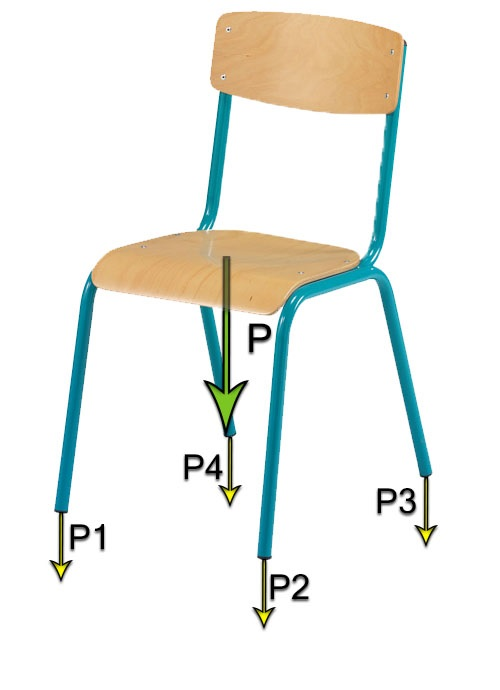
\includegraphics[scale=1]{image/Chaise_forces_homo.jpg}
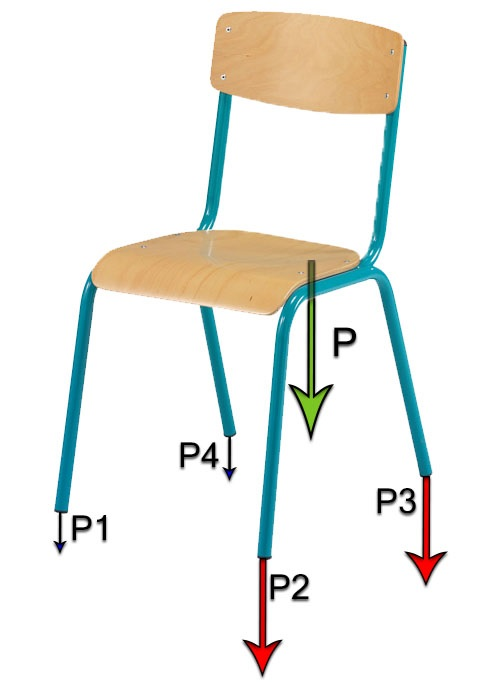
\includegraphics[scale=1]{image/Chaise_forces_hetero.jpg}
\end{center}
\caption{Illustration de la projection de la résultante des forces appliqués à la chaise vue au niveau des pieds de celle-ci pour deux position assises différentes}
\label{fig:illustr_chaise_forces}
\end{figure}

En pratique, on ne connais pas l'emplacement du point d'application de la force sur le plateau de la chaise. Or c'est déterminer sa position qui permet de définir la qualité de l'assise. Une bonne assise donnera une répartition des masses donnée et donc une position de la force totale donnée. Par exemple dans la figure \ref{fig:illustr_chaise_forces}, l'image de gauche correspond à quelqu'un qui serait assis bien droit au centre de la chaise tandis que l'image de droite correspond à quelqu'un assis (ou penché) du coté gauche de la chaise.

Cependant, connaissant la position de chaque pieds, et connaissant la valeur de la force appliquée à chaque pied, on peut trouver la position du barycentre des forces (c'est à dire, la position de la force totale et donc celle du centre de masse). 

Nous allons voir comment résoudre ce problème. Nous rappelons que le but est de déterminer la position du centre de masse, caractéristique de la posture.

Ici on considère le poids (c'est à dire les forces liés à la masse). Le barycentre des forces obtenus correspond donc au centre de masse. 
Par la suite, nos calculs se feront en 2 dimensions dans le plan du sol. En effet, on assimile les pieds de la chaise à des points du plan. On place un point $O$ origine du repère dans le plan. 

Pour chaque pieds de la chaise on associe les grandeurs suivantes:

\begin{enumerate}
\item un numéro $i$
\item un point du plan $A_i=(x,y)$ avec $x,y$ ses coordonnées
\item une valeur de force notée $m_i$ (par analogie à la masse)
\item un vecteur position $\vec{OA_i}$ représentant la position du point par rapport au point $O$
\end{enumerate}

L'idée ici est de représenter la chaise dans le plan du sol. La figure \ref{fig:schem_plan_sol_math} illustre une chaise carrée dont les quatre pieds sont projetés dans le plan du sol.


\begin{figure}[htbp]
\begin{center}
\begin{tikzpicture}
\coordinate (O) at (0,0);
\coordinate (A1) at (1,1);
\coordinate (A3) at (1,4);
\coordinate (A2) at (4,1);
\coordinate (A4) at (4,4);
\coordinate (X) at (5,0);
\coordinate (Y) at (0,5);

\draw[->] (-1,0) -- (X);
\draw (X) node[right] {$x$};
\draw [->] (0,-1) -- (Y);
\draw (Y) node[above] {$y$};
\draw (O) node[below left] {$O$} node{$\bullet$};
\draw (A1) node[below] {$A_1,m_1$} node{$\bullet$};
\draw (A2) node[below] {$A_2,m_2$} node{$\bullet$};
\draw (A3) node[above] {$A_3,m_3$} node{$\bullet$};
\draw (A4) node[above] {$A_4,m_4$} node{$\bullet$};
\end{tikzpicture}
\end{center}
\caption{Représentation de la chaise dans le plan du sol}
\label{fig:schem_plan_sol_math}
\end{figure}

Alors, on peut trouver $\vec{OG}$, vecteur position du barycentre des forces, par la formule \eqref{eq:centre_gravite}  suivante:

\begin{equation}
\label{eq:centre_gravite_vectorielle}
\vec{OG} = \frac{1}{M} \sum_i m_i  \cdot \vec{OA_i} =   \frac{1}{\sum_i m_i} \sum_i m_i  \cdot \vec{OA_i} 
\end{equation}

Avec $G$ qui est le point du barycentre, $M=\sum_i m_i$ est la somme des forces associés aux pieds.

L'équation \eqref{eq:centre_gravite_vectorielle} est vectorielle c'est à dire qu'elle est valide pour les coordonnées $(x_G,y_G)$ du point $G$.

C'est à dire qu'on a les relations \eqref{eq:centre_gravite_cartesienne}.

\begin{equation}
\label{eq:centre_gravite_cartesienne}
x_G = \frac{1}{M} \sum_i m_i  \cdot x_{A_i} \Leftrightarrow  y_G = \frac{1}{M} \sum_i m_i  \cdot y_{A_i}
\end{equation}

On peut donc retrouver la position du centre de masse d'une personne assise sur une chaise rien qu'en connaissant la valeur des forces au niveau de chaque pieds. La figure \ref{fig:schem_plan_sol_math_G} illustre le résultat qu'on pourrait obtenir pour le point $G$ avec une répartition des forces hétérogènes sur les pieds de la chaise.

\begin{figure}[htbp]
\begin{center}
\begin{tikzpicture}
\coordinate (O) at (0,0);
\coordinate (A1) at (1,1);
\coordinate (A3) at (1,4);
\coordinate (A2) at (4,1);
\coordinate (A4) at (4,4);
\coordinate (X) at (5,0);
\coordinate (Y) at (0,5);
\coordinate (G) at (1.7,3.3);
\coordinate (xG) at (1.7,0);
\coordinate (yG) at (0,3.3);

\draw[->] (-1,0) -- (X);
\draw (X) node[right] {$x$};
\draw [->] (0,-1) -- (Y);
\draw (Y) node[above] {$y$};
\draw (O) node[below left] {$O$} node{$\bullet$};
\draw (A1) node[below] {$A_1,m_1$} node{$\bullet$};
\draw (A2) node[below] {$A_2,m_2$} node{$\bullet$};
\draw (A3) node[above] {$A_3,m_3$} node{$\bullet$};
\draw (A4) node[above] {$A_4,m_4$} node{$\bullet$};

\draw [-] [dashed] (G) -- (xG);
\draw [-] [dashed] (G) -- (yG);

\draw (xG) node[below] {$x_G$} node{$.$};
\draw (yG) node[left] {$y_G$} node{$.$};

\draw (G) node[above right] {$G,M$} node[blue]{$\bullet$};
\end{tikzpicture}
\end{center}
\caption{Exemple de la position du centre de masse $G$ avec les valeurs de forces $m_i$ réparties de façon hétérogène sur les points $A_i$ }
\label{fig:schem_plan_sol_math_G}
\end{figure}

Nous avons donc évoqué toutes les raisons qui ont motivé le choix de mesurer des forces au niveau des pieds d'une chaise pour déterminer la position d'une personne.

L'idée, pour savoir si une personne est mal assise, est d'enregistrer la position du centre de masse lorsque la personne est bien assise. On peut ensuite comparer la position à un instant $t$ quelconque pour savoir si la personne est bien assise.

\textbf{Transition:} On sait maintenant que l'essentiel du projet consiste à acquérir la valeur des forces sous les pieds de la chaise. La partie suivante de ce rapport sera donc consacré à la réalisation de cette acquisition à l'aide de capteurs de forces et d'un Arduino.

\section{Le matériel et Arduino}
\label{chap:arduino}

Construire un correcteur de posture assise a nécessité de trouver un moyen de récupérer les informations de l'assise de l'utilisateur. On a vu dans la section \ref{chap:posture_determination} pourquoi cela est utile. Nous avons choisi de suivre la proposition de M.Beaufils qui était d'utiliser des capteurs positionnés sous les pieds d'une chaise. Il a été nécessaire d'utiliser un dispositif capable de mesurer les valeurs rapportées par ces capteurs. Notre choix se porte sur la proposition de M.Beaufils qui est d'utiliser un  micro-contrôleur Arduino Uno auquel sont connecté les capteurs de forces. 

Les premières séances de travail ont été consacré à des recherches sur les capteurs de forces (leurs caractéristiques et comment il fonctionnent). 

Nous avons appris pendant nos recherches que les capteurs de forces sont des résistances variables. La valeur de leur résistance varie en fonction de la force appliquée. Il existe cependant des capteurs pour lesquels la variation de résistances en fonction de la force appliquée est de l'ordre du Ohm $\Omega$ (typiquement des FSR, Force Sensitive Resistor) et d'autres pour lesquels la variation est de l'ordre du $\mu \Omega$ ou $\mathrm{m} \Omega$.

Un micro-contrôleur comme un Arduino possèdes des entrées sur lesquels il peut lire des valeurs de tensions par rapport à la masse. En effet, les pins allant de A0 à A5 sont des entrées analogiques sur lesquels on peut connecter une tension de 0 à 5V mesurable par l'Arduino. 

Avec un capteur qui se comporte comme une résistance variable, on peut confectionner un montage diviseur de tension permettant d'obtenir une tension mesurable par l'Arduino. Ce montage revient à connecter une résistance de valeur connue (on a choisit R1=10k$\Omega$) en série avec la résistance R variable du capteur et mesurer la tension aux bornes de la résistance connue.  En appliquant une tension de 5V fournie par l'Arduino au diviseur de tension, on a donc la relation suivante:

\begin{equation}
\label{eq:fsr_resistor}
U_{Capteur}= \frac{R_1}{ R + R_1} U_{Arduino} 
\end{equation}
 
 Avec $U_{Capteur}$ la tension entre la masse et le pin A0 de l'Arduino et $U_{Arduino}=5V$.
 
Au démarrage du projet nous n'avions aucune connaissance concernant les capteurs et l'Arduino. Nous avons donc expérimenté avec un capteur de force de type FSR et des potentiomètres pour simuler des capteurs dont la résistance varie selon la charge. Nous nous sommes rendu compte que le FSR est un capteur qui a une résistance presque infinie au repos et qui tend vers 0 lorsque le capteur est écrasé au maximum par une force. Nous avons alors constaté que l'Arduino peut lire des valeurs de tension entre 0V lorsqu'aucune force n'est appliquée et 5V lorsque le capteur est écrasé au maximum (ce qui vérifie l'équation \eqref{eq:fsr_resistor}).

Nous avons pu expérimenter avec des montages composé de 3 potentiomètres et d'un FSR connectés à l'Arduino pour faire des tests et apprendre à manipuler les données recueillies.

Nous nous sommes vite rendu compte qu'utiliser des FSR pour mesurer la répartition des masses sous les pieds d'une chaise ne serait pas adapté. En effet, le capteur sature au delà d'une pression de 2kg. Il est tout à fait possible de faire saturer le capteur avec nos doigts.

Dans un premier temps cette solution nous a convenus pendant que nous développions le microgiciel de l'Arduino et les applications PC et Android que nous vous présenterons par la suite dans le chapitre \ref{chap:Application}. La figure \ref{fig:arduino_v0} présente le montage que nous avons utilisé jusqu'à la séance 6 de travail.

\begin{figure}[htbp]
\begin{center}
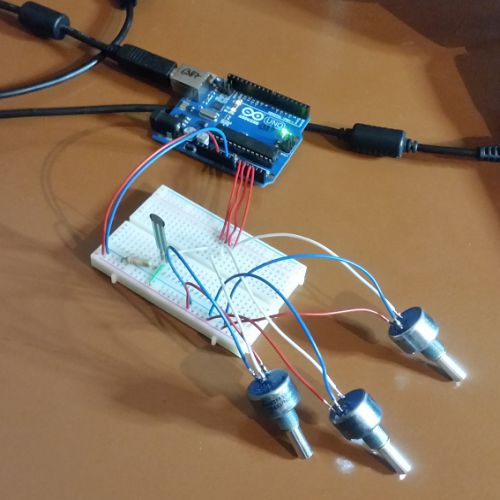
\includegraphics[scale=0.6]{image/Arduino_v0.jpg}
\end{center}
\caption{3 potentiomètres et une résistance de force connectés à un Arduino Uno}
\label{fig:arduino_v0}
\end{figure}

En parallèle du développement logiciel, nous avons recherché une alternative aux FSR pour connaître la force sous les pieds de la chaise. 

Nous avons appris qu'il existe des capteurs appelés \textit{cellule de charge} permettant de mesurer très précisément une force. En effet, les cellules de charges sont des capteurs utilisés dans les pèses-personnes électroniques et des balances électroniques. Certains sont tellement précis qu'ils sont utilisés en laboratoire pour mesurer les quantités de produits chimique avec une précision de l'ordre du milligramme.

Nous allons vous expliquer comment ils fonctionnent et comment nous les avons utilisé pour se projet.

Le fonctionnement d'une cellule de charge se base sur la capacité qu'ont les conducteurs électriques à voir leur résistance changer lorsqu'ils sont déformés. Les conducteurs réalisant cette fonction s'appellent des jauges de contrainte (ou \textit{strain gauge} en anglais). Le principe est d'utiliser un matériau déformable et de fixer une ou plusieurs jauge de contrainte sur celui-ci au niveau des zones de déformation. Ainsi les jauges de contraintes vont suivre la déformation du matériau et changer de résistance. La figure \ref{fig:load_cell_sparkfun} illustre ces propos en montrant comment on la déformation d'un morceau de métal déforme aussi les jauges de contraintes (petit morceau de fil conducteur en zig-zag).

\begin{figure}
\begin{center}
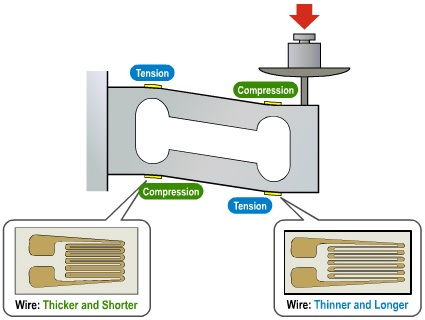
\includegraphics[scale=1]{image/load_cell.jpg}
\end{center}
\caption{Schéma d'une cellule de charge avec jauge de contrainte SOURCE: SPARKFUN.COM}
\label{fig:load_cell_sparkfun}
\end{figure}

Au niveau des zones de compression la résistance est plus faible et au niveau des zone de tensions (ou d'étirement) elle est plus grande.

En effet, on a la formule de la résistance $R$ avec $\rho$ la résistivité du matériau conducteur, $l$ sa longueur et $S$ sa section: 

\begin{equation}
R= \rho \frac{l}{S}
\end{equation}

Si la jauge de contrainte est compressée, sa longueur $l$ diminue et sa section $S$ augmente. On a donc $R$ qui diminue.

Au contraire, si la jauge de contrainte est étirée, la longueur $l$ augmente et sa section $S$ diminue. On peut imagine un élastique qu'on étire, il s'amincit et s'allonge lorsqu'on l'étire.  On a donc $R$ qui augmente.

Seulement, vous l'aurez compris, les allongements et modifications de la section des jauges de contraintes sont très faibles si matériau sur lequel est construit la cellule de charge se déforme peu. Ces variations se produisent à une échelle du nanomètre et les variations de résistances résultantes sont donc de l'ordre du $m\Omega$ ou du $\mu\Omega$. Ce sont de ces capteurs que nous parlions au début de cette section du rapport.

Avec un Arduino, on ne peut pas mesurer les variations de résistances avec un simple montage diviseur de tension. Il est alors nécessaire d'introduire un montage appelé le pont de WheatStone permettant de transformer la mesure de la résistance en une mesure de tension (cf. figure \ref{fig:wheatstone_bridge}). Cependant, malgré le pouvoir amplificateur
du pont WheatStone, les variations de tensions sont trop faibles (de l'ordre du $mV$) pour être mesurés directement par l'Arduino. Il a donc été nécessaire en plus du pont de WheatStone d'utiliser un amplificateur pour cellule de charge.

\begin{figure}
\begin{center}
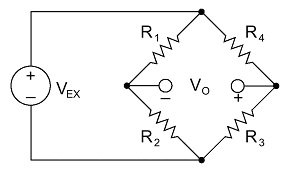
\includegraphics[scale=1]{image/wheatstone_bridge.jpg}
\end{center}
\caption{Schéma d'un pont de Wheatstone avec $V_{EX}$ la tension d'alimentation et $V_O$ la tension de sortie SOURCE:NATIONAL INSTRUMENT}
\label{fig:wheatstone_bridge}
\end{figure}

Jérémy a réussi à récupérer les cellules de charges d'un pèse personne électronique. Ceux-ci sont connecté en demi pont de Wheatstone et utilisent seulement 2 jauges de contraintes. La figure \ref{fig:load_sensor} à quoi ressemble ces capteurs. Ceci veut dire que ces capteurs fournissent seulement les résistance $R_1$ et $R_2$ dans la figure \ref{fig:wheatstone_bridge}. Sur ces capteurs, les valeurs  de $R_1$ et $R_2$ sont d'environ 1$k\Omega$.

\begin{figure}
\begin{center}
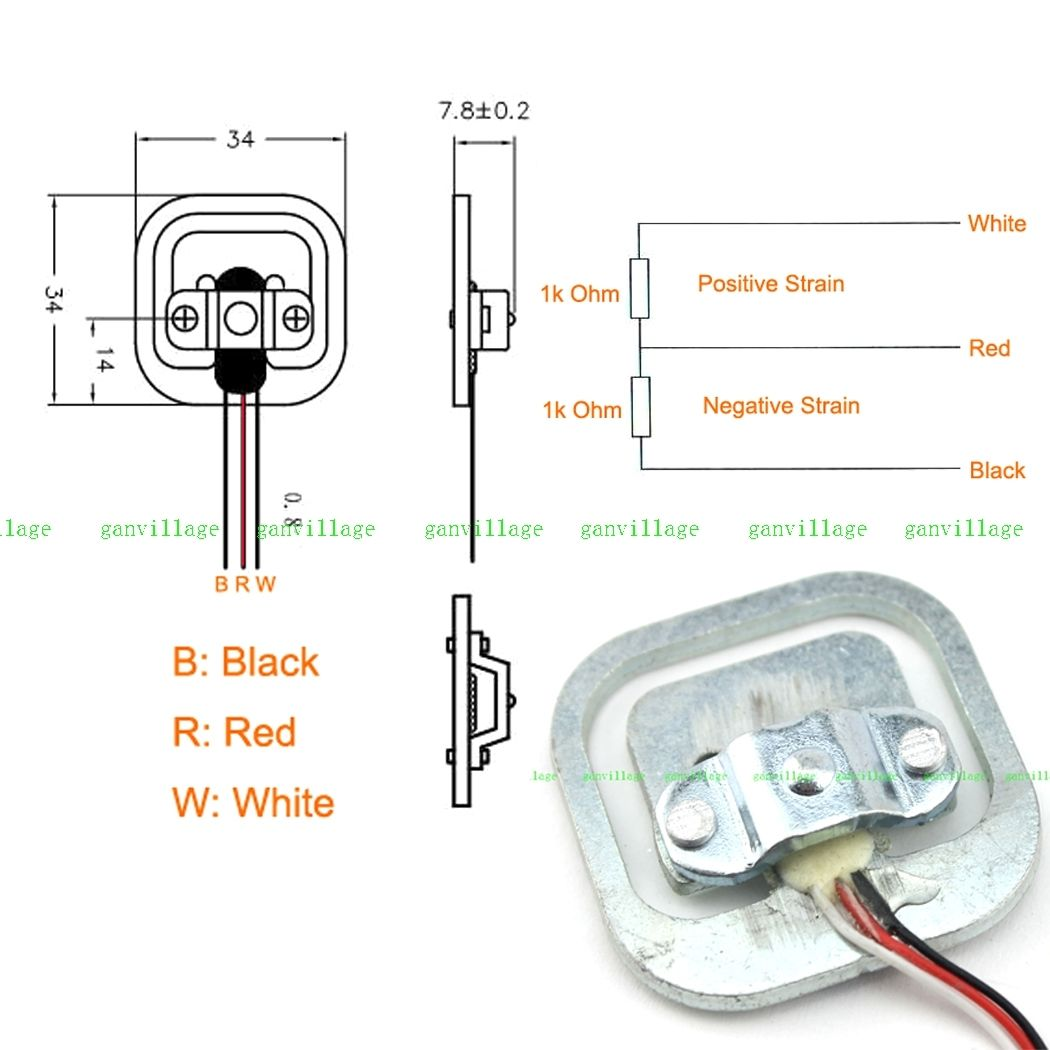
\includegraphics[scale=0.2]{image/load_sensor.jpg}
\end{center}
\caption{Schéma d'une cellule de charge avec jauge de contrainte SOURCE:ELECTRONIC STACK EXCHANGE}
\label{fig:load_sensor}
\end{figure}

Par la suite, le défi a été de réaliser 4 ponts de Wheatstone en couplant chaque cellules de charges à 2 résistances de 1$k\Omega$. Typiquement, on a placé 2 résistances fixes de $1k\Omega$ au niveau de $R_4$ et $R_3$.  On a pu ensuite connecter ces cellules de charges à des amplificateurs HX711 (cf. figure \ref{fig:load_sensor_connected}) pour obtenir un signal compatible avec l'Arduino.

\begin{figure}
\begin{center}
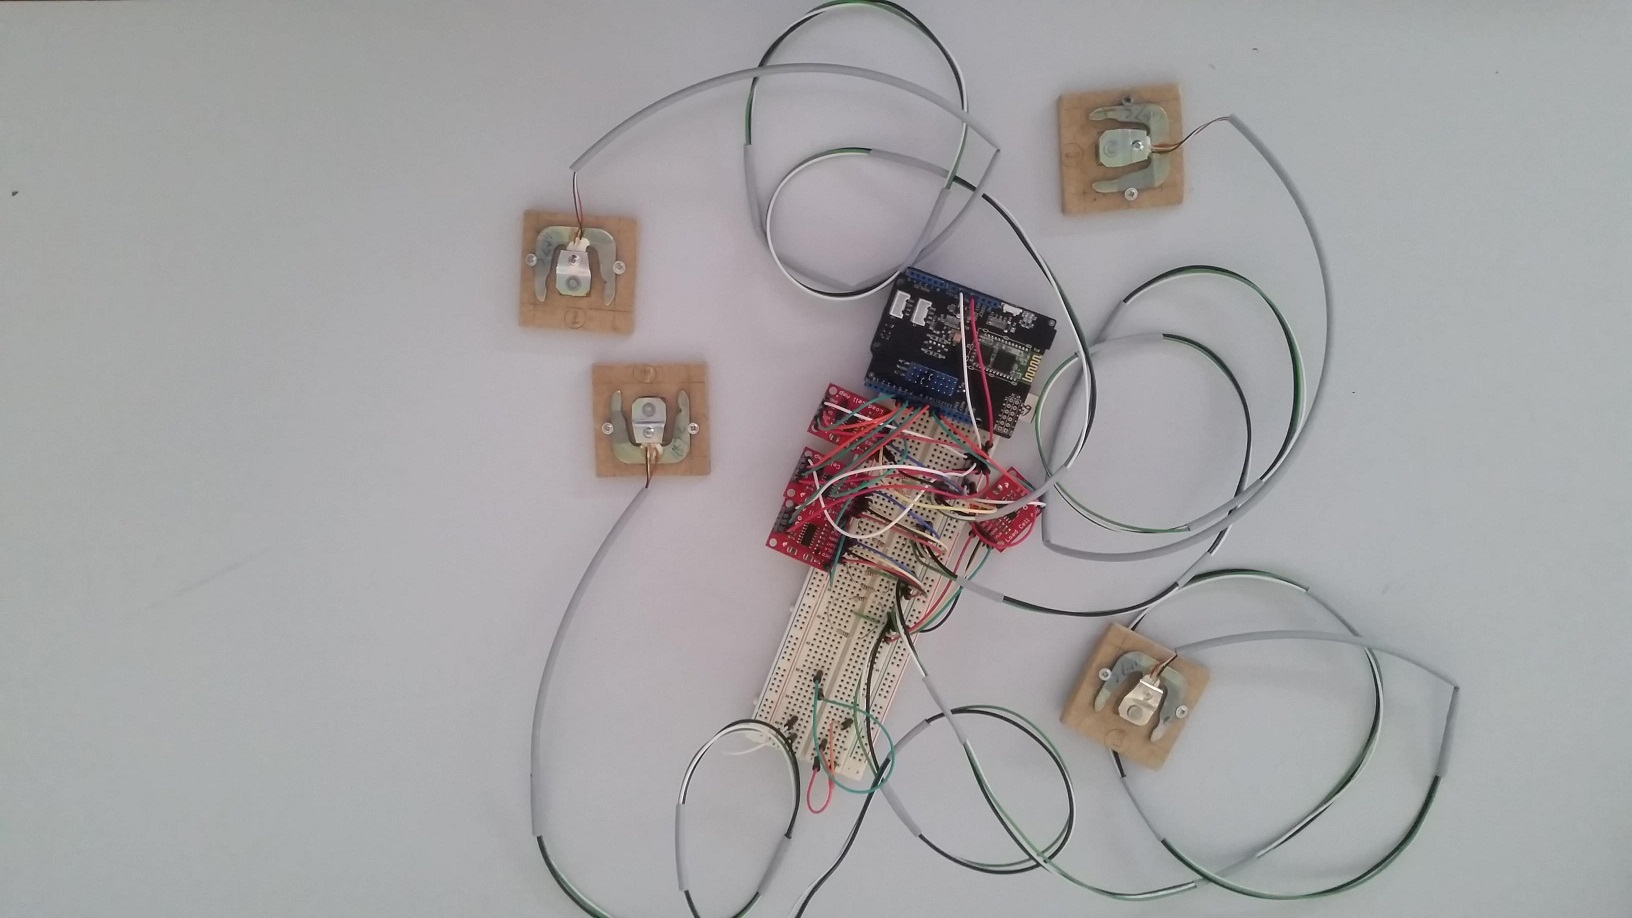
\includegraphics[scale=0.2]{image/load_sensor_connected.jpg}
\end{center}
\caption{4 cellules de charges en demi-pont connectées à l'Arduino en utilisant des amplis HX711}
\label{fig:load_sensor_connected}
\end{figure}

 En effet, les amplificateurs prennent un pont de wheatstone en entrée. On a donc connecté nos ponts de Wheatstone complet a l'amplificateur HX711 et connecté les amplis à l'Arduino au niveau des pins digitales. Les HX711 fournissent $V_{EX}$ et analysent $V_O$. L'amplificateur va d'une part amplifier le signal (la tension $V_O$) du pont mais aussi le convertir en signal numérique (digital) directement lisible par l'Arduino. Lors de la programmation de l'Arduino, nous avons donc utilisé une librairie permettant de contrôler et analyser les données de l'amplificateur HX711.

Nous avons désormais fait le tour du matériel que nous avons étudié et utilisé pour réaliser ce projet. Nous allons maintenant nous intéresser à l'aspect logiciel de ce projet qui consiste d'une part à programmer l'Arduino pour qu'il lise les valeurs des capteurs de forces et d'autre part à communiquer avec une interface utilisateur (un Smartphone ou un PC) pour donner les résultats et l'interprétation à l'utilisateur.

\chapter{Le développement du logiciel}
\label{chap:logiciel}

En parallèle de la conception de l'électronique du correcteur de posture, nous avons travailler sur un programme de visualisation de la posture de l'utilisateur. Nous avons beaucoup travaillé avec la version \ref{fig:arduino_v0} pour développer le logiciel de l'Arduino et l'interface graphique sur PC et Android. Lorsque la commande des amplificateurs HX711 et des cellules de charges est arrivé, nous avons simplement modifié très légèrement le logiciel de l'Arduino pour qu'il utilise les amplificateurs au lieu des potentiomètres de la version \ref{fig:arduino_v0}. Le fonctionnement général des 2 versions (potentiomètres et amplis) est similaire et ne diffère que dans la façon d'initialiser les capteurs et récupérer la valeur des capteurs. Les données récupéré seront identiques et l'interprétation donnée par les deux versions est la même.

Commençons donc par la programmation de l'Arduino et la gestion des capteurs.

%Une fois que la partie électronique du correcteur de posture est réalisée, et que donc les capteurs fournissent une tension mesurable à l'Arduino, il est temps de passer au développement du logiciel qui va nous permettre de visualiser la posture de l'utilisateur. Ce développement commence, évidemment, au niveau de l'Arduino.

\section{Bas niveau : l'Arduino}
\label{sec:logiciel_bas}

Le langage de programmation utilisé pour programmer l'Arduino est peu différent de C ou C++; en fait, il est basé sur ces langages. Le code, après quelques petits changements, est compilé par un compilateur \texttt{avr-g++} (compilateur C/C++). Pour le programme de l'Arduino, nous avons choisi d'utiliser surtout la syntaxe C ; nous avons toutefois utilisé aussi quelques fonctions C++ pour rendre notre programme plus efficace. Nous avons donc utilisé l'EDI Arduino (Environnement de développement informatique) officiel disponible à l'adresse \url{https://www.arduino.cc/} gratuitement. Cet environnement nous a permis d'écrire du code C et C++ et de le télé-verser dans la mémoire de l'Arduino. Il possède aussi des fonctions intéressantes tels qu'un moniteur série permettant d'avoir un endroit où on peut afficher des messages envoyés par l'Arduino.

Le but du programme de l'Arduino est de récupérer les données que fournissent les amplificateurs à partir des cellules de charge, de les traiter afin de n'avoir que des valeurs valides, et enfin de les envoyer (que ce soit par USB ou par Bluetooth) à l'application (que ce soit l'application PC ou celle d'Android).

En travaillant avec la version utilisant des potentiomètres, on pouvait récupérer les valeurs des potentiomètres en éxecutant la commande \texttt{AnalogRead(A\#)} avec \textbf{\#} le numéro du pin Analog sur lequel on a connecté le potentiomètre. On se rappelle que l'entrée au niveau du pin Analog est un montage diviseur de tension. Ce montage fournis comme on l'a vu dans le chapitre précédent \ref{chap:arduino} une tension entre 0 et 5V au niveau du pin Analog. La commande  \texttt{AnalogRead(A\#)} permet de convertir cette valeur de tension en un nombre entier compris entre 0 et 1023 (donc 1024 valeurs possibles).

Dans la version utilisant les amplificateurs, on a utilisé la librairie HX711 (\url{https://github.com/bogde/HX711}) permettant de récupérer les valeurs des capteurs sur les pins digitals de l'Arduino. 
Cette fois on récupère le nombre entier à l'aide de la commande \texttt{sensor.get\_unit()} ou \texttt{sensor.get\_value()} (\texttt{sensor} est l'objet représentant l'ampli dans le code C). 
Sans calibration de l'amplificateur, ce nombre est brut et n'a pas de sens. 
On applique alors des corrections notamment en faisant le zéro des amplificateurs avec la commande \texttt{sensor.tare()}.
 \'A ce moment, la valeur retournée par l'amplificateur augmentent de manière linéaire avec la force appliqué au capteur (elle a donc du sens).

\'Etant donné qu'on a fabriqué des demi-ponts de Wheatstone, ils sont sensibles aux variations de températures et la valeur des capteurs peut fluctuer. 
La valeur donnée par les amplificateurs a donc tendance à fluctuer (les fluctuations sont de l'ordre de \textpm 5) et peut parfois prendre des valeurs négatives par rapport au zéro obtenu par la tare.
 Pour essayer de compenser ce problème, premièrement, on a pris la valeur absolue des valeurs (on supprime alors les fluctuations négatives). 
En effet, l'idée derrière cette correction est que lorsque le capteur ne peux avoir que des valeurs positives ou nulles.
 La valeur nulle est la valeur au repos et la valeur augmentera lorsque une force sera appliqué sur le capteur.
  Un deuxième correction a été d'ajouter un décalage (offset) des valeurs obtenus pour faire en sorte de ne jamais avoir 0. 
  Comme on a montré avec la formule \eqref{eq:centre_gravite_vectorielle}, si les valeurs des capteurs sont toutes nulles en même temps, la position du centre de gravité sera $(0, 0)$. 
  Or on a voulu que, lorsque les capteurs sont au repos (donc après une tare), le centre de gravité coïncide avec le centre de la chaise.
   Pour cela, il faut impérativement que peut importe la géométrie de la chaise, les valeurs au niveau des capteurs soient non nulles.


% D'abord, donc, on récupère les données en faisant un \textit{read} sur les capteurs; on enregistre ces valeurs à un tableau de quatre entiers (\texttt{int}), après avoir pris leur valeur absolue, et avoir fait un \textit{offset}. Ceci est nécessaire, car les petites variations de température entre les cellules de charge donnent naissance à des variations de tension, qui sont ensuite amplifiées. Pour corriger ce paramètre, il est nécessaire de prendre la valeur absolue des données fournies par les capteurs de charge (en réalité, il est impossible qu'une personne applique une force négative aux capteurs !). Ensuite, pour vérifier que la valeur minimale des capteurs ne sera jamais 0 pour tous les capteurs, on prend soin de décaler les valeurs obtenues; comme on a montré avec la formule \ref{eq:centre_gravite_vectorielle}, si les \guillemotleft\ masses \guillemotright\ des capteurs sont tous nuls en même temps, la position du centre de gravité sera $(0, 0)$. Au cas où aucune charge n'est appliquée aux capteurs, le centre de gravité doit coïncider avec le centre de la chaise.

Une fois ce travail achevé, on envoie les données à l'application. On sera en mode série, ce qui implique qu'on enverra les données octet par octet. Il est évident que cette option sert à mettre à jour les données en temps réel, en assurant en même temps une faible éventualité de pertes d'information ou de données incomplètes.
%, étant donné qu’on envoie un seul octet à la fois.
Un périphérique utilisant une liaison série possède voies de communication. La première est la voie RX permettant de recevoir les données (octets). La seconde est la voie TX permettant de transmettre les données.  Si on veux faire dialoguer deux périphérique série, il faut connecter la voie TX et RX de l'un respectivement sur les voies RX et TX de l'autre.

\begin{eqnarray}
TX_1 \rightarrow RX_2
\\
RX_1 \leftarrow TX_2
\end{eqnarray}

Ainsi les données envoyées par l'un sont reçu par l'autre et vis-versa. Ce mode de connexion est dit \guillemotleft croisé \guillemotright .
Cependant pour que deux périphériques séries communiquent entre-eux, il faut qu'ils parlent le même langage c'est à dire que les paramètres de communication soient les même.

On commence donc en initialisant la communication série, ce qui veut dire qu'on doit choisir les paramètres de communication. Afin d'obéir aux standards de l'Arduino, nous avons fixé les paramètres de communication de la façon suivante :

\begin{itemize}
\item \textit{BaudRate} (vitesse de communication) : 9600 bauds
\item \textit{DataBits} (nombre de bits de données) : 8
\item \textit{StopBits} (nombre de bits de stop) : 1
\item \textit{Parity} (parité du message) : NO\_PARITY (pas de parité)
\end{itemize}

Pour tous ces paramètres, hormis le premier, nous avons choisi de suivre les standards mis en place par l'Arduino : 8 bits de données, 1 bit de stop, et pas de parité de message.
Tout les périphériques séries utilisés pour communiquer ( l'Arduino, le PC, le smartphone Android, le module bluetooth) sont configurés de cette façon de manière à ce que tous se comprennent.
 %Pour la communication, nous avons choisi un \texttt{baud rate} de 9600, car nous voulons que la communication se passe rapidement, mais pas au point de nous donner des résultats incohérents, dans le cas où sont impliqués des appareils ou des ordinateurs différents. En choisissant 9600 bauds, on obtient une vitesse confortable et une bonne compatibilité tant en Bluetooth qu'en USB.

Pour transmettre les données on a utilisé le port USB B intégré à l'Arduino. La connexion est donc directe entre le PC et l'Arduino. Le PC reconnais alors l'Arduino en tant que périphérique de communication série et on peut dialoguer sans problème. On a donc le schéma suivant pour la communication USB.

\begin{eqnarray}
TX_{Arduino-USB} \rightarrow RX_{PC}  \\
RX_{Arduino-USB}  \leftarrow TX_{PC}
\end{eqnarray}

Pour effectuer une liaison série en Bluetooth, on a utilisé un shield Bluetooth car l'Arduino ne possède pas de module bluetooth installé en usine. Le shield bluetooth un circuit électronique comprenant un module bluetooth conçu pour l'Arduino et venant se connecté sur celui-ci. En fait, le module bluetooth communique avec l'Arduino via le protocole série et le module bluetooth communique en série avec la carte bluetooth du PC ou du smartphone. On a donc le schéma suivant pour la communication Bluetooth.

\begin{eqnarray}
TX_{Arduino-Digital} \rightarrow RX_{Shield-Digital} \rightarrow TX_{Shield-Bluetooth} \rightarrow RX_{PC/Smartphone}  \\
RX_{Arduino-Digital} \leftarrow TX_{Shield-Digital} \leftarrow RX_{Shield-Bluetooth} \leftarrow TX_{PC/Smartphone}
\end{eqnarray}

On a donc utilisé deux pins digital de l'Arduino pour communiquer en série avec le Shield. 
Ainsi l'Arduino est connecté physiquement au module bluetooth et le module bluetooth est connecté sans fil au PC ou smartphone. 
On voit bien avec ce schéma que le shield bluetooth est un intermédiaire. 
Les données envoyés par l'arduino (sur la voie TX du port digital) se retrouvent bien sur la voie TX du bluetooth.
 De même les données arrivant sur la voie RX du bluetooth se retrouvent bien sur la voie RX de l'Arduino.
  Il a fallu suivre ce diagramme lors de la programmation et de la configuration des différents pins utilisés pour la communication série car on peut rapidement se tromper.

Une fois qu'on a initialisé la communication, on peut envoyer les données. Nous rappelons que le but est d’envoyer les 4 différentes valeurs obtenues à partir des 4 capteurs. Avant même de discuter le processus de l'envoi des données des capteurs, on sait qu'on doit envoyer un caractère qui \textit{initialise} le message, ainsi qu’un autre qui le \textit{termine}. Ceci sert à distinguer les messages entre eux, et à vérifier que toutes les données sont bien transmises. Pour initialiser le message, on envoie un caractère ASCII \guillemotleft\ STX \guillemotright\ (start of text), qui a pour code le nombre décimal 2. Pour terminer le message, on envoie un caractère \guillemotleft\ CR \guillemotright\ (enter/carriage return), qui a pour code le nombre décimal 13. Notre module de communication sur l'application (qu'elle soit en PC ou en téléphone portable) est avertie désormais que les données des capteurs seront comprises entre ces deux caractères.

%Pour l'envoi des données des capteurs, nous avons décidé que le meilleur message serait court et simple.
%Ainsi, on diminue encore plus le danger de transmettre ou de recevoir des données incomplètes, car on envoie le minimum absolu des caractères. FAUX ne pas mettre
Comme on ne connaît pas la taille de la valeur de chaque capteur (c'est-à-dire le nombre des chiffres), on ne peut pas les envoyer directement l'un après l'autre, il nous faut donc un séparateur.
Nous avons choisi un caractère point-virgule (\guillemotleft ; \guillemotright), car il offre une séparation visuelle mais aussi sémantique. Toutefois, pour cette application n'importe quel caractère pourrait être choisi comme séparateur tant que ce n'est pas un chiffre ou un caractère délimiteur (STX ou CR). Le format de chaque message est donc le suivant :

\begin{center}
\texttt{STX (02)}\\
\texttt{valeur1;valeur2;valeur3;valeur4}\\
\texttt{CR (13)}
\end{center}

%où \texttt{02} et \texttt{13} sont les caractères \texttt{STX} et \texttt{CR} respectivement, et \texttt{valeur1, valeur2, valeur3, valeur4} sont les nombres entiers obtenues à partir des 4 capteurs. 
où \texttt{valeur1, valeur2, valeur3, valeur4} sont des chaines de caractères ASCII représentant les nombre entiers/valeurs des capteurs. 
%Comme on l'a dit plus haut, les valeurs sont transmises caractère par caractère, et non pas toutes en même temps.

%Finalement, afin d'éviter d'envoyer des données qui ne changent pas (ou alors qui changent très peu), nous avons mis en place un petit \guillemotleft timer \guillemotright , qui fait qu'on envoie des données tous les 100 millisecondes.
Finalement, nous avons décidé d'envoyer ces données toutes les 100 millisecondes pour avoir une mesure réactive de la posture. Il a donc fallu implémenter un pause c'est à dire un \guillemotleft timer \guillemotright  dans l'envoie des données.
 Une implémentation de premier niveau consisterait à arrêter le programme pour 100 millisecondes avant d'envoyer à nouveau des données, mais elle n'est pas tout a fait correcte.
  Si, pendant le temps d'arrêt, on veut avoir accès aux données, ou par exemple envoyer des commandes à l'Arduino à partir de l'application PC ou Android, il risque d'y avoir des problèmes, car le programme sera en pause pendant ce temps-là.
   Pour éviter ce problème, nous avons implémenté la fonctionnalité de manière \textit{asynchrone} : on calcule la différence entre le temps dit \guillemotleft du début \guillemotright\ et le temps dit \guillemotleft actuel \guillemotright . 
   Si cette différence est supérieur ou égale à 100 millisecondes, on lit les données à partir des capteurs et on les envoie, puis on met à jour le temps dit \guillemotleft du début \guillemotright . 
   Cela nous permet d'avoir accès aux autres fonctionnalités de l'Arduino, en limitant en même temps les données envoyés.


\textbf{Transition:} Nous avons pu voir comment nous avons choisis de récupérer les données des capteurs et les transmettre à l'ordinateur ou le smartphone qui va se charger de la visualisation. Intéressons-nous sans attendre aux programmes PC et Android que nous avons conçu pour permettre à l'utilisateur de visualiser sa posture.

\section{Haut niveau : les applications PC et Android}
\label{sec:logiciel_haut}

Pour gérer les données fournies par les load sensors, nous devons construire une application qui visualise la posture assise de l'utilisateur. Pour le développement de cette application, nous avons choisi \texttt{Java} comme langage de programmation, car il est conforme avec cette tâche, et il nous est accessible à travers notre cursus académique; en réalité, tous les deux nous l'avions déjà utilisé, aussi bien pour les projets PeiP de la première année, que pour des projets personnels.

Pour mieux organiser notre workflow et afin d'avoir accès aux versions précédentes de notre logiciel, nous avons utilisé \texttt{git} comme \textit{VCS} (logiciel de contrôle des versions). Suite à la création d'un dépôt sur \texttt{GitHub}, nous avons pu synchroniser nos fichiers locaux, gérés par \texttt{git}, sur le dépôt en ligne. Cela permet de mettre en jour le projet, et \guillemotleft\ télécharger \guillemotright\ les changements qu'on y fait, avec une seule commande.

Pour que notre application soit plus fonctionnelle, nous avons décidé de mettre en place une version PC et Android. De cette manière, on permet à l'utilisateur,selon sa préférence, de consulter le correcteur de posture depuis son ordinateur ou son téléphone portable.

Le design général de l'application dans les deux cas reste le même, indépendamment de la plateforme : il y a une partie dédiée à la visualisation de la chaise, et une autre partie dédiée à la configuration (qu'elle concerne la chaise ou bien la visualisation). 

Dans la partie visualisation, le schème choisi représente tout d'abord les pieds de la chaise, symbolisés par des cercles auxquels s'associe un nombre, qui correspond au ID de chaque load sensor. Pour une chaise banale à quatre pieds, on aura donc quatre cercles, situés aux quatre coins du panel de visualisation, et portant des nombres 1, 2, 3 et 4. Le schèma de la visualisation comprend en outre le centre de gravité de la personne assise, qui est donné par la formule \eqref{eq:centre_gravite_vectorielle}. Le centre de gravité est représenté par un cercle noir, qui se déplace dans le panel de visualisation suivant les changements de la posture assise de l'utilisateur.

Finalement, le schèma comprend aussi la deadzone, c'est-à-dire la zone dans laquelle la posture assise est considérée idéale. Elle est représentée par un cercle vert, dont on peut modifier la taille ainsi que la position. Cela garantit que si on a une chaise différente (par exemple une chaise à trois ou à cinq pieds), l'utilisateur peut déplacer la position de la deadzone selon ses besoins : il suffit de prendre la posture considérée comme idéale, puis de calibrer la deadzone en cliquant sur le bouton correspondant.

En somme, le schème choisi permet les manipulations suivantes :
\begin{itemize}
\item Modifier le nombre et les positions des pieds de la chaise;
\item Modifier la position et la taille de la deadzone;
\item Sauvegarder la chaise;
\item Utiliser une chaise déjà enregistrée.
\end{itemize}


Pour utiliser l'application, il faut d'abord configurer la chaise. On clique sur le bouton \guillemotleft\ configuration \guillemotright\ , on saisit le nombre des pieds de la chaise et leurs positions (on supposera que pour une chaise à quatre pieds, le pied qui se trouve devant et à gauche est au point (0,0); cela veut dire que les positions des autres pieds seront mesurées relativement au point (0,0) qu'on a défini). Une fois que la chaise est configurée, on peut se connecter à l'Arduino, soit par Bluetooth (auquel cas on doit faire un \guillemotleft\ pair \guillemotright\  afin de pouvoir se connecter), ce qui est préférable, soit par USB. Finalement, on doit s'asseoir correctement, afin de calibrer l'application. On clique alors sur \guillemotleft\ tare \guillemotright\ , puis sur \guillemotleft\ calibrer \guillemotright\  pour calibrer la position de la deadzone. Une fois qu'on l'a calibrée, la deadzone est placée dans la position considérée comme \guillemotleft\ optimale \guillemotright\ . Finalement on peut modifier sa taille selon nos préférences. 

Maintenant, l'application affichera la deadzone et le barycentre, qui deviendra rouge quand il sort de la deadzone, ce qui veut dire que notre posture n'est pas bonne. En ce point, on peut sauvegarder la chaise afin d'éviter la procédure de configuration chaque fois qu'on veut utiliser l'application. Pour ce faire, on clique sur \guillemotleft\ sauvegarder chaise \guillemotright\ , puis on choisit un dossier et un nom pour notre chaise (la chaise sera sauvegardée dans un fichier \texttt{.txt}). La prochaine fois qu'on ouvrira l'application, on pourra cliquer sur \guillemotleft\ charger une chaise \guillemotright\  et donc charger le fichier qu'on a enregistré. Ce fonctionnement nous permet aussi d'utiliser plusieurs chaises sans avoir besoin de changer la configuration chaque fois qu'on utilise une chaise différente.


%% === COMPTES RENDUS ===
\weeklyreport{11/01/2017}{Rapport seance 1}
\weeklyreport{18/01/2017}{Rapport seance 2}
\weeklyreport{25/01/2017}{Rapport seance 3}
\weeklyreport{01/02/2017}{Rapport seance 4}
\weeklyreport{08/02/2017}{Rapport seance 5}
\weeklyreport{15/02/2017}{Rapport seance 6}
\weeklyreport{08/03/2017}{Rapport seance 7}
\weeklyreport{15/03/2017}{Rapport seance 8}
\weeklyreport{22/03/2017}{Rapport seance 9}
\weeklyreport{29/03/2017}{Rapport seance 10}
\weeklyreport{05/04/2017}{Rapport seance 11}
\weeklyreport{26/04/2017}{Rapport seance 12}


\chapter{SOURCES}
BROUILLON BIBLIOGRAPHIE
\url{https://www.arduino.cc/}


\end{document}


